\nonstopmode
%%*****************************************************************************
%% $Id: extex-users.tex 5326 2007-02-27 13:09:26Z gene $
%%*****************************************************************************
%% Author: Gerd Neugebauer
%%-----------------------------------------------------------------------------
\documentclass{extex-doc}

\usepackage{makeidx}

\title{\ExBib\ User's Guide}
\author{Gerd Neugebauer}

\newcommand\Arg[1]{\(\langle\){\tt\itshape #1}\(\rangle\)}
\newcommand\CLI[1]{\texttt{-#1}\index{#1@\texttt{-#1}}}
\newcommand\Property[1]{\texttt{#1}\index{#1@\texttt{#1}}}
\newcommand\File[1]{\texttt{#1}\index{#1@\textsf{#1}}}
\newcommand\Prog[1]{\texttt{#1}\index{#1}}
\newcommand\Mode[1]{\texttt{#1}\index{#1}}
\newcommand\macro[1]{\texttt{\char`\\ #1}\index{#1@\texttt{\char`\\ #1}}}
\newcommand\Macro[1]{\texttt{\char`\\ #1}}
\newcommand\tag[1]{%
    \(\langle\)\textit{#1}\(\rangle\)%
    \index{#1@\protect\Tag{#1}}}
\newcommand\Tag[1]{\texorpdfstring{%
    \(\langle\)\textit{#1}\(\rangle\)}{<#1>}}

\newenvironment{syntax}{%
  \begin{tabbing}\kern2em\=\kern2em\=\kill
  }{%
  \end{tabbing}}
\newcommand\SyntaxDef{\>\(\rightarrow\)\>}
\newcommand\SyntaxOr{\>\(|\)\>}

\def\setVersion$#1: #2 ${\gdef\Version{0.1 (Revision #2)}}
\setVersion$Revision: 5326 $

\def\n{\char`\\n}
\def\t{\char`\\t}

\providecommand\BibTeX{\textsc{Bib}\TeX}

\makeindex

\begin{document}%%%%%%%%%%%%%%%%%%%%%%%%%%%%%%%%%%%%%%%%%%%%%%%%%%%%%%%%%%%%%%%

\begin{titlepage}
  \parindent=0pt
  \begin{center}
  \vspace*{1pt}
  \vfill
  \ExBibbox
  \vfill
  \textsf{\bfseries\Huge User's Guide}
  \vfill
  \textsf{\Large Version \Version}
  \vfill
  \textsf{\large Gerd Neugebauer}
  \vfill
  \vfill
%\maketitle

  \begin{abstract}\parindent=0pt
    This document describes \ExBib. It explains how to get \ExBib\ up
    and running and which features \ExBib\ offers to you.

    The intended audience for this document are end users of a
    bibliography processor who want to use \ExBib\ on the command line or
    as plug-in replacement of \BibTeX.
  \end{abstract}
  \unitlength=1mm
  \begin{picture}(0,0)
    \put(56,120){\makebox(0,0){\scalebox{6}{\rotatebox{45}{\color{red}\textsf{\Huge\bfseries Draft}}}}}
  \end{picture}
  \end{center}
\newpage
\footnotesize
\copyright\ 2008 The \ExTeX\ Group and individual authors listed below 
\medskip

Permission is granted to copy, distribute and/or modify this document
under the terms of the GNU Free Documentation License, Version 1.2 or
any later version published by the Free Software Foundation. A copy of
the license is included in the section entitled ``GNU Free
Documentation License''.
\bigskip

This product includes software developed by the Apache Software
Foundation (http://www.apache.org/).

\vfill

Gerd Neugebauer\\
Im Lerchelsb\"ohl 5\\
64521 Gro\ss-Gerau (Germany)
\smallskip

\href{mailto://gene@gerd-neugebauer.de}{gene@gerd-neugebauer.de}

\end{titlepage}

\tableofcontents

%------------------------------------------------------------------------------
\chapter{Introduction}
%@author Gerd Neugebauer

\ExTeX{} aims at providing a high-quality typesetting system. The
development of \ExTeX\ has been inspired by the experiences with \TeX.
The focus lies on an open design and a high degree of configurability.

A tight integration of several components is one of the possibilities
opened by \ExTeX. To work into this direction \ExBib\ has been
implemented. It is a plug-in replacement for \BibTeX~0.99c\
\cite{btxdoc,btxhak} or \BibTeX~8.

\section{This Document}

This document is meant to be a reference document. It should contain
all information necessary to know. It is not meant to be a tutorial.
Thus do not expect tutorial type material in this document.


\section{Web Site}
%@author Gerd Neugebauer

There is a web site devoted to \ExTeX. \index{WWW}\index{Web Site}This
web site can be reached via the URL

\begin{quotation}
  \url{http://www.extex.org}
\end{quotation}


\section{Mailing Lists}
%@author Gerd Neugebauer

If you are ready to try \ExTeX{} you might as well want to join a
mailing list to get in contact with the community.\index{Mailing list}

\begin{quotation}
  \url{http://www.dante.de/listman/extex}
\end{quotation}


\section{Reporting Bugs}
%@author Gerd Neugebauer


If you find any bugs in \ExTeX\ you can submit them 
%either 
via a HTML form.
% or via email. 
You can find the HTML form at
\begin{quotation}
  \url{http://www.extex.org/bugs}
\end{quotation}
%Emails containing the description can be sent to
%\begin{quotation}
%  \href{mailto:extex-bugs@dante.de}{extex-bugs@dante.de}
%\end{quotation}

Please include in your description 
\begin{itemize}
\item the source of a \emph{minimal} example showing the problem
\item the log file resulting from running this example
\item a description why you think that something went wrong and what
  the expected result would be
\item a description of the environment you are using (host
  architecture, operating system, Java version)
\end{itemize}


%------------------------------------------------------------------------------
\chapter{Getting Started}
%@author Gerd Neugebauer

In this chapter we describe the steps you can take to get \ExTeX\ up
and running. We try to use as few as possible premises. Thus it should
be not too hard to get started.

\section{Prerequisites}
%@author Gerd Neugebauer

\subsection{Java}
%@author Gerd Neugebauer

You need to have Java 5\index{Java} or later installed on your
system. You can get Java for a several systems directly from
\url{java.sun.com}. Download and install it according to the
installation instructions for your environment.

To check that you have an appropriate Java on your path you can use
the command \texttt{java} with the argument \texttt{-version}. This
can be seen in the following listing:

\lstset{morecomment=[l]{\#}}%
\begin{lstlisting}{morecomment=[l][keywordstyle]{>}}
# java -version
java version "1.5.0_04"
Java(TM) 2 Runtime Environment, Standard Edition (build 1.5.0_04-b05)
Java HotSpot(TM) Client VM (build 1.5.0_04-b05, mixed mode)
#
\end{lstlisting}


\subsection{TEXMF}
%@author Gerd Neugebauer

If you want to use more than the pure \ExBib\ engine, fonts and macros
can be inherited from a texmf tree\index{texmf}. \ExBib\ itself does
not contain a full texmf tree. It comes just with some rudimentary
files necessary for testing. Thus you should have installed a texmf
tree, e.g. from a \TeX Live\index{TeXlive@\TeX Live} installation.
This can be found on the \href{http://www.ctan.org}{Comprehensive
  \TeX\ Archive Network (CTAN)}\index{CTAN}.

There is no need to install the texmf tree in a special place. You
have to tell \ExBib\ anyhow where it can be found. It is even possible
to work with several texmf trees.

One requirement for the texmf trees is that they have a file database
(\File{ls-R}). \ExBib\ can be configured to work without it, but then
\ExBib\ is deadly slow. Thus you do not really want to try this
alternative.


\section{Getting \ExBib}
%@author Gerd Neugebauer

\subsection{Getting the Installer}
%@author Gerd Neugebauer

The simplest way to get \ExBib\ up and running is to use the \ExBib\ 
installer. This installer\index{installer} is distributed as one file
\File{ExBib-setup.jar}. You can download it from

\begin{quotation}
  \url{http://www.extex.org/download/}
\end{quotation}

If you have got the installer there is no need for you to get the
sources as well. Thus you can skip the following section.


\subsection{Getting the Sources}
%@author Gerd Neugebauer

The sources of \ExTeX\ are stored in a Subversion repository. To access this
repository you need access to the internet and Subversion installed in some
way.


The coordinates of the repository are:\index{repository}\index{CVS}
\medskip
\begin{quotation}
  \texttt{https://svn.berlios.de/svnroot/repos/extex}
\end{quotation}
\bigskip

We assume here that you have access to Subversion on the command line.
This can be either a shell on a Unix-like system or something like
cygwin on Windows. We also assume that you have direct connection to
the internet or Subversion configured to access the repository on the
internet.

First we create a directory where the sources are stored:
\begin{lstlisting}{}
# mkdir ExBib
\end{lstlisting}

Next we change the current directory to this base directory:
\begin{lstlisting}{}
# cd ExBib
\end{lstlisting}

Finally we can check out the sources:
\begin{lstlisting}{}
# svn checkout https://svn.berlios.de/svnroot/repos/extex/trunk/ExBib
\end{lstlisting}

This command shows a lot of output. At the end the current directory
contains the sub-directory \texttt{trunk} which is filled with a lot
of files and directories.


\section{Installing \ExBib}
%@author Gerd Neugebauer

There are several ways to install \ExBib.
The easiest installation of \ExBib\ works with the \ExBib\ installer.
This installer is named \File{ExBib-setup.jar}. You can start the
installer with the following command line:\index{installer}

\begin{lstlisting}{}
# java -jar ExTeX-setup.jar
\end{lstlisting}

On Windows\index{Windows} with a properly installed Java\index{Java}
you can also start the installer by double-clicking
\texttt{ExBib-setup.jar} in the Explorer\index{Explorer}.

\begin{figure}[t]
  \centering
  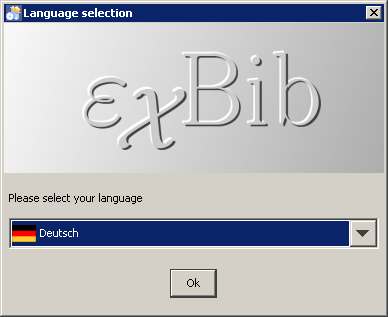
\includegraphics[width=.8\textwidth]{img/inst1}
  \caption{The Language Selection in the Installer}

  \label{fig:inst1}
\end{figure}
The installer provides a graphical user interface with a wizard
guiding you through the installation process. The first dialog is
shown in figure~\ref{fig:inst1}. As you can see you can select one of
several languages for the installation process. Currently the
languages English and German are supported. There might be some more
at the time you are performing the
installation.\index{installer!language}\index{language!installer}

Note that the internationalization covers the installer only. \ExBib\
can be run under different language environments as well. This is
controlled by a setting at run-time. Currently only an English
language binding for \ExBib\ is provided.\index{language}

Finally you have to make sure that the executables \Prog{exbib} or
\Prog{exbib.bat} is on your path for executables.\index{path}


\subsection{Replaying an Installation}
%@author Gerd Neugebauer

Sometimes it is desirable to perform an installation on several
similar machines. This means that the answers to the questions in the
installer are the same. This process can be automated.
\begin{figure}[tp]
  \centering
  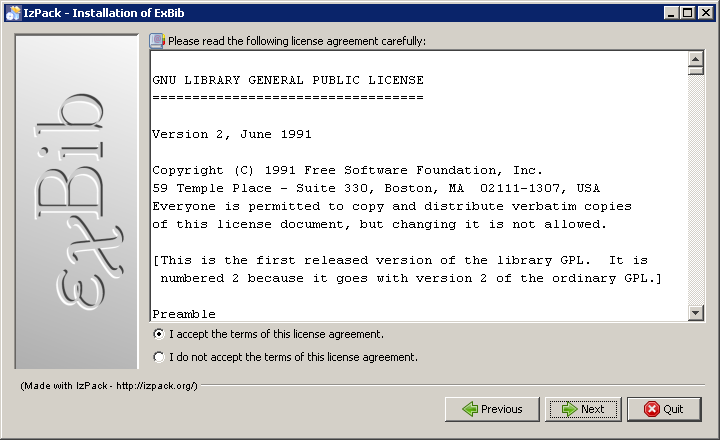
\includegraphics[width=.8\textwidth]{img/inst4}
  \caption{Generating a Auto-Configuration for the Installer}
  \label{fig:inst8}
\end{figure}

In figure~\ref{fig:inst8} you can see the last screen of the
installer. Here you have the possibility to select the button
``Generate an automatic installation script''. This produces an XML
file which can be passed to the installer to avoid the
dialogs.\index{installer}\index{installation script}

Suppose you have named the file \texttt{replay.xml} in the file
selector which pops up when the button has been pressed. Then you can
replay the installation with the following command invocation:

\begin{lstlisting}{}
# java -jar ExBib-setup.jar replay.xml
\end{lstlisting}

This supposes that the two files \File{ExTeX-setup.jar} and
\texttt{replay.xml} are in the current directory.
Finally you have to make sure that the executables \Prog{extex} or
\Prog{extex.bat} is on your path for executables.\index{path}


%------------------------------------------------------------------------------
\section{Configuring \ExTeX}
%@author Gerd Neugebauer

The behaviour of \ExTeX\ can be influenced via command line arguments
and configuration files. Most of the times the start-up files will be
enough for the casual user.


\subsection{Start-up Files}
%@author Gerd Neugebauer

Whenever \ExTeX\ starts it looks for start-up files named
\File{.extex}. This file is sought in the user's home directory in the
current directory. The settings in the current directory overwrite the
settings from the user's home directory. Those in turn overwrite the
built-in settings.

\ExTeX\ user properties files contain setting of properties. This is
done in a line-based way. Lines containing only white space characters
are ignored. If the first character is a hash sign (\verb|#|) then the
line is treated as a comment and ignored.

The first appearance of a equal sign (\verb|=|) or the colon
(\verb|:|) separates the name of the property from the value. Leading
and trailing white space is ignored both for the name and the value of
the property.

Some characters have a special meaning. The backslash (\verb|\|) acts
as an escape character. The sequence \verb|\n| is replaced by the
newline character. If the last character in a line is a backslash then
the line is continued in the next line. To produce a single backslash
it has to be doubled.

You can set any property name you like to a legal value. \ExTeX\ will
not complain about unknown properties but ignore them silently.
The following properties are used by \ExTeX:

\begin{description}
\item[\Property{extex.code}]\ \\
  This parameter contains \ExTeX\ code to be executed directly. The
  execution is performed after any code specified in an input file.

   Example:\index{relax@\texttt{\char`\\relax}}
\begin{lstlisting}{}
  extex.code = \\relax
\end{lstlisting}

\item[\Property{extex.color.converter}]\ \\
  This parameter contains the logical name of the color converter to
  use. The color converter describes how colors are converted between
  different color soaces. Currently at least the color spaces RGB,
  Grayscale, HSV, and CMYK are supported.
  The configuration mapps this to a concrete instance.

  Example:
\begin{lstlisting}{}
  extex.color.converter = basic
\end{lstlisting}

\item[\Property{extex.config}]\ \\
  This parameter contains the name of the configuration resource to
  use. This configuration resource is sought on the class path.

  Example:
\begin{lstlisting}{}
  extex.config = tex.xml
\end{lstlisting}

\item[\Property{extex.encoding}]\ \\
  This parameter contains the name of the property for the standard
  encoding to use.

  Example:
\begin{lstlisting}{}
  extex.encoding = ISO-8859-1 
\end{lstlisting}

\item[\Property{extex.error.handler}]\ \\
  This parameter contains the logical name of the error handler.

  Example:
\begin{lstlisting}{}
  extex.error.handler = TeX
\end{lstlisting}

\item[\Property{extex.fonts}]\ \\
  This parameter contains the property indicating where to find font
  files. The value is a path similar to \Property{extex.texinputs}.

  Example:
\begin{lstlisting}{}
  extex.fonts = /usr/local/share/fonts
\end{lstlisting}

\item[\Property{extex.halt.on.error}]\ \\
  This boolean parameter contains the property indicating whether
  the processing should stop after the first error. Allowed values are
  \verb|true| and \verb|false|.

  Example:
\begin{lstlisting}{}
  extex.halt.on.error = false
\end{lstlisting}

\item[\Property{extex.file}]\ \\
  This parameter contains the file to read from. It has no default. If
  this property is not set or set to the empty string then no attempt
  is made to read a file. Maybe the user is asked to provide one.

  Example:
\begin{lstlisting}{}
  extex.file = abc.tex
\end{lstlisting}

\item[\Property{extex.format}]\ \\
  This parameter contains the name of the format to read. An empty
  string denotes that no format should be read. This is the default.
  In this case \ExTeX\ acts with no macros or fonts preloaded.

  Example:
\begin{lstlisting}{}
  extex.format = plain
\end{lstlisting}

\item[\Property{extex.ini}]\ \\
  If set to \verb|true| then act as ini\TeX. In this case no format
  has to be preloaded. All parameters are set to the "`factory
  settings"'. Allowed values are \verb|true| and \verb|false|.

  Example:
\begin{lstlisting}{}
  extex.ini = true
\end{lstlisting}

\item[\Property{extex.interaction}]\ \\
  This parameter contains the interaction mode. Possible values are
  the numbers 0\dots3 and the symbolic names \Mode{batchmode} (0),
  \Mode{nonstopmode} (1), \Mode{scrollmode} (2), and
  \Mode{errorstopmode} (3).

  Example:
\begin{lstlisting}{}
  extex.interaction = scrollmode
\end{lstlisting}

\item[\Property{extex.jobname}]\ \\
  This parameter contains the name of the job. It is overwritten if a
  file is given to read from. In this case the basename of the input
  file is used instead. If no file is read in then the default value
  \verb|texput| is used.

  Example:
\begin{lstlisting}{}
  extex.jobname = texput
\end{lstlisting}

\item[\Property{extex.jobname.master}]\ \\
  This parameter contains the name of the job to be used with high
  priority.

  Example:
\begin{lstlisting}{}
  extex.jobname.master = texput
\end{lstlisting}

\item[\Property{extex.lang}]\ \\
  This parameter contains the name of the locale to be used for the
  messages. The value is a two letter ISO language code.  \ExTeX\ can
  be internationalized just by providing some files with the translated
  strings. Currently only the language English (\verb|en|) is
  supported.

  Example:
\begin{lstlisting}{}
  extex.lang = en
\end{lstlisting}

\item[\Property{extex.nobanner}]\ \\
  This parameter contains a boolean indicating that the banner should
  be suppressed. Allowed values are \verb|true| and \verb|false|.

  Example:
\begin{lstlisting}{}
  extex.nobanner = false
\end{lstlisting}


\item[\Property{extex.output}]\ \\
  This parameter contains the output format. This logical name is
  resolved via the configuration.

  Example:
\begin{lstlisting}{}
  extex.output = pdf
\end{lstlisting}

\item[\Property{extex.output.directories}]\ \\
  This parameter contains the list of directories where output files should be
  created. The period is interpreted as the current directory. The
  default is the current directory only.

  Example:
\begin{lstlisting}{}
  extex.output.directories = .:/tmp
\end{lstlisting}

\item[\Property{extex.progname}]\ \\
  This parameter can be used to overrule the name of the program shown
  in the banner and the version information.

  Example:
\begin{lstlisting}{}
  extex.progname = iniExTeX
\end{lstlisting}

\item[\Property{extex.stacktrace.on.internal.error}]\ \\
  This parameter can be used to force a stack trace on stdout if an
  internal error is encountered. This is handy for development.
  Allowed values are \verb|true| and \verb|false|.

  Example:
\begin{lstlisting}{}
  extex.stacktrace.on.internal.error = true
\end{lstlisting}

\item[\Property{extex.texinputs}]\ \\
  This parameter contains the additional directories for searching
  \ExTeX\ input files.
  The directories are separated by the system-dependant separator.
  This separator is a colon (\verb|:|) on Unix\index{Unix} and the semicolon
  (\verb|;|) on Windows\index{Windows}.

  Example:
\begin{lstlisting}{}
  extex.texinputs = /home/gene/lib/tex
\end{lstlisting}

\item[\Property{extex.trace.input.files}]\ \\
  This boolean parameter contains the indicator whether or not to
  trace the search for input files.  Allowed values are \verb|true|
  and \verb|false|.

  Example:
\begin{lstlisting}{}
  extex.trace.input.files = false
\end{lstlisting}

\item[\Property{extex.trace.font.files}]\ \\
  This boolean parameter contains the indicator whether or not to
  trace the search for font files.  Allowed values are \verb|true| and
  \verb|false|.


  Example:
\begin{lstlisting}{}
  extex.trace.font.files = false
\end{lstlisting}

\item[\Property{extex.trace.macros}]\ \\
  This boolean parameter contains the indicator whether or not to
  trace the execution of macros.  Allowed values are \verb|true| and
  \verb|false|.

  Example:
\begin{lstlisting}{}
  extex.trace.macros = false
\end{lstlisting}

\item[\Property{extex.trace.tokenizer}]\ \\
  This boolean parameter contains the indicator whether or not to
  trace the work of the tokenizer.  Allowed values are \verb|true| and
  \verb|false|.

  Example:
\begin{lstlisting}{}
  extex.trace.tokenizer = false
\end{lstlisting}

\item[\Property{extex.typesetter}]\ \\
  This parameter contains the name of the typesetter to use. If it is
  not set then the default from the configuration file is used.

  Example:
\begin{lstlisting}{}
  extex.typesetter = default
\end{lstlisting}

\end{description}


\subsection{Configuration Files}
%@author Gerd Neugebauer

Configuration files of another kind contain the assembly instructions
for \ExTeX. Those files can be used to provide additional features in
\ExTeX. 

\INCOMPLETE

%------------------------------------------------------------------------------
\section{Running \ExTeX}
%@author Gerd Neugebauer

Currently \ExTeX\ can be run from the command line. In this respect it
is more or less identical to \TeX\ and can be used as a plug-in
replacement.

The following sample show a simple invocation of \ExTeX\ without any
command line arguments.

{\lstset{morecomment=[l]{*}}%
\begin{lstlisting}{}
# extex
This is ExTeX, Version 0.0 (TeX compatibility mode)
**\relax

*\end

No pages of output.
Transcript written on ./texput.log.
\end{lstlisting}}

In this case \ExTeX\ enters interaction with the user and asks for an
input file. This is indicated by the two asterisks. We have entered
\macro{relax} here to indicate that we are not willing to pass in a
file name. The \ExTeX\ system asks us to enter some command --
indicted by the single asterisk. Here we have entered \macro{end} to
indicate that we want to finish the processing. Thus \ExTeX\ 
terminates normally.

\INCOMPLETE

{\lstset{morecomment=[l]{*}}%
\begin{lstlisting}{}
# extex plain
This is ExTeX, Version 0.0 (TeX compatibility mode)
(plain Preloading the plain format: codes, registers, parameters, fonts,
more fonts, macros, math definitions, output routines, hyphenation(hyphen))
*\dump
Beginning to dump on file plain.fmt

*\end

No pages of output.
Transcript written on ./plain.log.
\end{lstlisting}}


\subsection{Command Line Parameters}
%@author Gerd Neugebauer

The invocation of the executable \Prog{extex} can be controlled by
large number of command line arguments. Those command line arguments
are described in the following list:

\begin{description}
\item[\Arg{code}]\ \\
  This parameter contains \ExTeX\ code to be executed directly. The
  execution is performed after any code specified in an input file. On
  the command line the code has to start with a backslash. This
  restriction does not hold for the property settings.

  This command line argument sets the property \Property{extex.code}
  
\item[\Arg{file}]\ \\
  This parameter contains the file to read from. A file name may not
  start with a backslash or an ambercent. It has no default.

  This command line argument sets the property \Property{extex.file}.
  
\item[\CLI{-} \Arg{file}]\ \\
  This parameter terminates the normal processing of arguments. The
  next argument -- if present -- is interpreted as input file. With
  this construction it is possible to process an input file which
  starts with one of the special characters \verb|\| or \verb|&|.

  This command line argument sets the property \Property{extex.file}
  if a file argument is present.

\item[\CLI{configuration} \Arg{resource}]\ \\
  This parameter contains the name of the configuration resource to
  use. This configuration resource is sought on the class path.
  
  This command line argument sets the property \Property{extex.config}.
  
\item[\CLI{copyright}]\ \\
  This command line option produces a copyright notice on the standard
  output stream and terminates the program afterwards.

\item[\tt\&\Arg{format}]\index{\&}
\item[\CLI{fmt} \Arg{format}]\ \\
  This parameter contains the name of the format to read. An empty
  string denotes that no format should be read. This is the default.

  This command line argument sets the property \Property{extex.format}.
  
\item[\CLI{debug} \Arg{spec}]\ \\
  This command line parameter can be used to instruct the program to
  produce debugging output of several kinds. The debug output is
  written to the log file. The specification \Arg{spec} is interpreted
  left to right. Each character is interpreted according to the
  following table:

  \begin{tabular}{lp{.4\textwidth}l}\toprule
    \textit{Spec}& \textit{Description}& \textit{See} \\\midrule
    F& 	This specifier contains the indicator whether or not to trace
    the searching for input files. & 	\Property{extex.trace.input.files}\\
    f& 	This specifier contains the indicator whether or not to trace
    the searching for font files.&      \Property{extex.trace.font.files}\\
    M& 	This specifier contains the indicator whether or not to trace
    the execution of macros.&	 	\Property{extex.trace.macros}\\
    T& 	This specifier contains the indicator whether or not to trace
    the work of the tokenizer.& 	\Property{extex.trace.tokenizer}\\
    \bottomrule
  \end{tabular}

  The following example shows a possible invocation with this
  parameter: 
\begin{lstlisting}{}
# extex -debug FfMT abc.tex
This is ExTeX, Version 0.0 (TeX compatibility mode)
...
\end{lstlisting}
  
\item[\CLI{halt-on-error}]\ \\
  This parameter contains the indicator whether the processing should
  halt after the first error which has been encountered.

  This command line argument sets the property \Property{extex.halt.on.error}.
  
\item[\CLI{help}]\ \\
  This command line option produces a short usage description on the
  standard output stream and terminates the program afterwards.
  
\item[\CLI{ini}]\ \\
  If set to true then act as ini\TeX.\index{initex@ini\TeX} In this
  case no format has to be preloaded. All parameters are set to the
  "`factory settings"'.

  This command line argument sets the property \Property{extex.ini}.

  The following example shows a possible invocation with this
  parameter: 
\begin{lstlisting}{}
# extex -ini abc.tex
This is ExTeX, Version 0.0 (TeX compatibility mode)
...
\end{lstlisting}
  
\item[\CLI{interaction} \Arg{mode}]\ \\
  This parameter contains the interaction mode. possible values are
  the numbers 0\dots3 and the symbolic names \Mode{batchmode} (0),
  \Mode{nonstopmode} (1), \Mode{scrollmode} (2), and
  \Mode{errorstopmode} (3).

  This command line argument sets the property \Property{extex.interaction}.
  
  The following example shows a possible invocation with this
  parameter:
\begin{lstlisting}{}
# extex -interaction batchmode abc.tex
This is ExTeX, Version 0.0 (TeX compatibility mode)
...
\end{lstlisting}

\item[\CLI{job-name} \Arg{name}]\ \\
  This parameter contains the name of the job. It is overwritten if a
  file is given to read from. In this case the base name of the input
  file is used instead.

  This command line argument sets the property \Property{extex.jobname}.
  
\item[\CLI{language} \Arg{language}]\ \\
  This parameter contains the name of the locale to be used for the
  messages.

  This command line argument sets the property \Property{extex.lang}.
  
\item[\CLI{output} \Arg{format}]\ \\
  This parameter contains the output format. This logical name is
  resolved via the configuration.

  This command line argument sets the property \Property{extex.output}.

  The following example shows a possible invocation with this
  parameter: 
\begin{lstlisting}{}
# extex -output pdf abc.tex
This is ExTeX, Version 0.0 (TeX compatibility mode)
\end{lstlisting}
  
\item[\CLI{progname} \Arg{name}]\ \\
  This parameter can be used to overrule the name of the program shown
  in the banner and the version information.  The following example
  shows a possible invocation and the resulting output:

\begin{lstlisting}{}
# extex -progname XeTxE -version
This is XeTxE, Version 0.0 (1.4.2_06)
#
\end{lstlisting}

  This command line argument sets the property \Property{extex.progname}.
  
\item[\CLI{texinputs} \Arg{path}]\ \\
  This parameter contains the additional directories for searching
  \ExTeX\ input files.  The directories are separated by the
  system-dependant separator.  This separator is a colon (\verb|:|) on
  Unix\index{Unix} and the semicolon (\verb|;|) on
  Windows\index{Windows}.
  
  This command line argument sets the property
  \Property{extex.texinputs}.
  
\item[\CLI{texmfoutputs} \Arg{dir}]\ \\
  This parameter contains the name of the property for the fallback if
  the output directory fails to be writable.
  
  This command line argument sets the property
  \Property{extex.outputdir.fallback}.
  
\item[\CLI{texoutputs} \Arg{dir}]\ \\
  This parameter contain the directory where output files should be
  created.

  This command line argument sets the property \Property{extex.outputdir}.
  
\item[\CLI{version}]\ \\
  This command line parameter forces that the version information is
  written to standard output and the program is
  terminated.\index{version} The version of \ExTeX\ is shown and the
  version of the Java engine\index{Java} in parentheses. The following
  example shows a possible invocation and the resulting output:

\begin{lstlisting}{}
# extex -version
This is ExTeX, Version 0.0 (1.4.2_06)
#
\end{lstlisting}
\end{description}

Command line parameters can be abbreviated up to a unique prefix --
and sometimes even more. Thus the following invocations are
equivalent:

\begin{verbatim}
  extex -v
  extex -ve
  extex -ver
  extex -vers
  extex -versi
  extex -versio
  extex -version  
\end{verbatim}



%------------------------------------------------------------------------------
\bibliographystyle{alpha}
\bibliography{references}

%------------------------------------------------------------------------------
{\scriptsize\printindex}

\end{document}%%%%%%%%%%%%%%%%%%%%%%%%%%%%%%%%%%%%%%%%%%%%%%%%%%%%%%%%%%%%%%%%%
%
% Local Variables: 
% mode: latex
% TeX-master: nil
% End: 
